\documentclass[journal]{IEEEtran}

% ---- Safe, minimal packages (ASCII only) ----
\usepackage[T1]{fontenc}
\usepackage[utf8]{inputenc}
\usepackage{lmodern}
\usepackage{graphicx}
\usepackage{amsmath,amssymb}
\usepackage{booktabs}
\usepackage{siunitx}
\usepackage[hidelinks]{hyperref}
\usepackage{cite}

\graphicspath{{./}{figs/}}

\title{A Comparative Review of DRAM and FeRAM: The Boundary between Volatile and Non-Volatile Memory and Future Perspectives}

\author{Shinichi~Samizo%
\thanks{S. Samizo is with Project Design Hub (Samizo–AITL), Japan. E-mail: \texttt{samizo-aitl@example.org}.}
}

\markboth{Draft for IEEE-style submission}{Samizo: DRAM vs FeRAM Comparative Review}

\begin{document}
\maketitle

\begin{abstract}
Dynamic Random-Access Memory (DRAM) is the workhorse of volatile memory, while ferroelectric memories (FeRAM and FeFET) offer CMOS-compatible non-volatility. This paper reviews DRAM and FeRAM from technology scaling and reliability to system-level use. We summarize key metrics (speed, retention, endurance, and energy/bit) and discuss hybrid hierarchies that combine DRAM performance with FeRAM persistence.
\end{abstract}

\begin{IEEEkeywords}
DRAM, FeRAM, FeFET, HfO2, retention, endurance, scaling, memory hierarchy.
\end{IEEEkeywords}

\section{Introduction}
\section{Introduction}

In the late 1990s, Japan's semiconductor industry was in transition. At Epson's Sakata 8-inch fab, DRAM was \emph{not} pursued as an end business; rather, DRAM technology transfer was used as a \textbf{strategic vehicle} to absorb submicron process technologies at and beyond 0.35~\si{\micro\meter} and redeploy them into Epson's core devices (ASICs, logic ICs, display drivers, and inkjet driver ICs).

The technology transfer from Mitsubishi covered three nodes, each with a clear role:
(1) 0.5~\si{\micro\meter} 16~Mbit DRAM --- to establish mass-production capability and stabilize fab operation; 
(2) 0.35~\si{\micro\meter} 64~Mbit DRAM (2nd gen) --- to introduce a scaled process while tackling yield window narrowing; 
(3) 0.25~\si{\micro\meter} 64~Mbit DRAM (3rd gen) --- as the next-stage validation bed and the basis for in-house deployment.

This paper focuses on the 0.25~\si{\micro\meter} (3rd gen) ramp-up in 1998: a process overview, the ramp-up method, and a failure-analysis–driven yield-improvement cycle. We also trace how these results enabled the 0.25~\si{\micro\meter} mobile pseudo-SRAM (VSRAM) in 2001 and why trench-based 0.18~\si{\micro\meter} VSRAM was abandoned.


\section{DRAM Technology and Scaling}
DRAM technology progressed via high-k dielectrics, deep trench or stacked capacitors, and continual process innovations. A key challenge is to maintain sufficient capacitance while suppressing leakage and variability at extremely small dimensions \cite{choi2022}. Device and array proposals investigate capacitor aspect-ratio increases and layout optimizations, yet refresh power and timing margins remain system concerns \cite{kim2021_dram}.

To extend scaling, the community studies directions analogous to 3D NAND, such as stacking capacitor arrays or exploring 3D DRAM architectures. These ideas may relieve planar density pressure but add significant integration complexity and do not remove the need for refresh \cite{iedm2023_dram}. From a metric viewpoint, DRAM offers sub-ns class access, very low read energy per bit, and effectively unlimited endurance (refresh-limited rather than wear-out limited), but short data retention that mandates periodic refresh \cite{choi2022}.


\section{FeRAM Technology and Advances}
The discovery of robust ferroelectricity in doped HfO2 films enabled FeRAM and FeFET \cite{boscke2011,mueller2012}. FeFET cells provide 1T bit storage with non-volatility and fast reads; FeRAM capacitors offer low-voltage writes. Challenges include polarization variability, endurance in the 10^{12}–10^{13} range, and TDDB under high fields; recent work addresses device physics and integration routes toward memory and compute-in-memory.

\begin{figure}[!t]
  \centering
  \fbox{\rule{0pt}{1.10in}\rule{0.95\linewidth}{0pt}}
  \caption{Write energy per bit vs. write speed (placeholder). FeRAM/FeFET often sit at higher write energy than DRAM but provide non-volatility.}
  \label{fig:energy_speed}
\end{figure}


\section{Comparative Analysis: DRAM vs FeRAM}
\label{sec:comparison}
\label{sec:comparison}

Table~\ref{tab:comparison} summarizes representative literature values for DRAM and FeRAM. 
DRAM provides high speed and very low energy/bit but requires periodic refresh due to short intrinsic retention~\cite{choi2022,kim2021_dram,iedm2023_dram}. 
FeRAM offers non-volatility with retention beyond $10^{5}$\,s and endurance reported in the $10^{12}$--$10^{13}$ range for optimized HfO$_2$ stacks, 
typically at higher write energy per bit~\cite{boscke2011,mueller2012,noheda2023,martin2020}.

\begin{table}[!t]
\centering
\caption{Representative metrics (order-of-magnitude, literature indications).}
\label{tab:comparison}
\scriptsize
\begin{tabular}{lcccc}
\toprule
Tech. & Speed (ns) & Retention (s) & Endurance & Energy/bit \\
\midrule
DRAM  & $\le 10$  & $\sim 10^{-2}$ to $10^{-1}$ & $\ge 10^{16}$ & $10$--$100$ fJ \\
FeRAM & $\le 50$  & $\ge 10^{5}$                & $10^{12}$--$10^{13}$ & $10^{2}$--$10^{3}$ fJ \\
\bottomrule
\end{tabular}
\end{table}

% ===== Figure 1: Speed (access time) vs retention =====
\begin{figure}[!t]
\centering
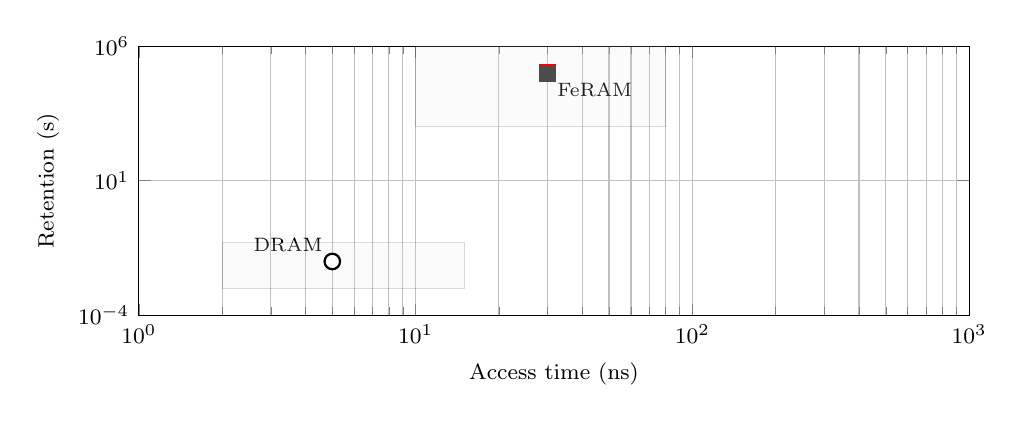
\begin{tikzpicture}
\begin{loglogaxis}[
  width=\linewidth,
  height=5.0cm,
  xlabel={Access time (ns)},
  ylabel={Retention (s)},
  xmin=1e0, xmax=1e3,
  ymin=1e-4, ymax=1e6,  % ★修正: 10^{-4}~10^{6}
  grid=both,
  label style={font=\footnotesize},
  tick label style={font=\footnotesize},
  clip=false
]

% DRAM point
\addplot+[only marks, mark=*, mark size=2.8pt,
          mark options={fill=white,draw=black,thick}]
          coordinates {(5, 1e-2)};
\node[above left, font=\scriptsize] at (axis cs:5,1e-2){DRAM};

% FeRAM point
\addplot+[only marks, mark=square*, mark size=3.0pt,
          mark options={fill=black!70}]
          coordinates {(30, 1e5)};
\node[below right, font=\scriptsize] at (axis cs:30,1e5){FeRAM};

% DRAM region
\addplot [draw=black, fill=black!10, opacity=0.15]
coordinates {(2,1e-3) (15,1e-3) (15,5e-2) (2,5e-2)} -- cycle;

% FeRAM region
\addplot [draw=black, fill=black!10, opacity=0.15]
coordinates {(10,1e3) (80,1e3) (80,1e6) (10,1e6)} -- cycle;

\end{loglogaxis}
\end{tikzpicture}
\caption{Speed vs.\ retention trade-off. DRAM is faster but requires refresh, whereas FeRAM provides long retention at modest access times.}
\label{fig:speed_retention}
\end{figure}

% ===== Figure 2: Write energy vs write time =====
\begin{figure}[!t]
\centering
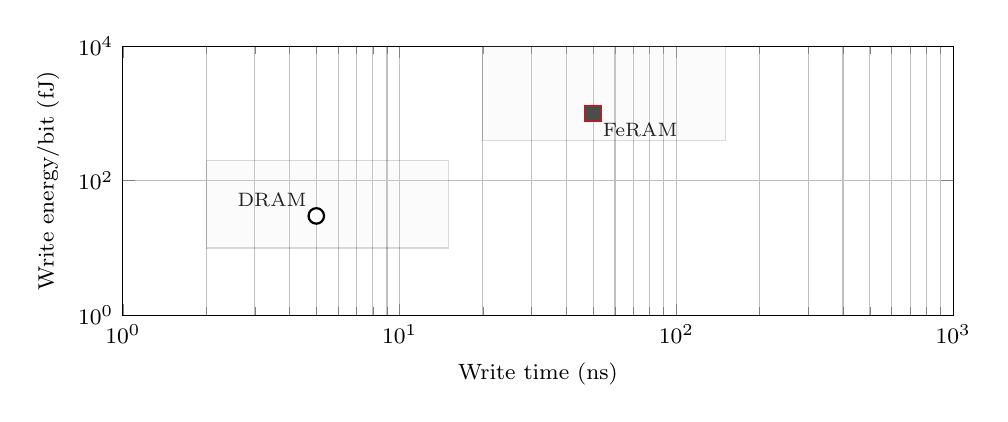
\begin{tikzpicture}
\begin{loglogaxis}[
  width=\linewidth,
  height=5.0cm,
  xlabel={Write time (ns)},
  ylabel={Write energy/bit (fJ)},
  xmin=1e0, xmax=1e3,
  ymin=1e0, ymax=1e4,  % ★修正: 10^{0}~10^{4}
  grid=both,
  label style={font=\footnotesize},
  tick label style={font=\footnotesize},
  clip=false
]

% DRAM point
\addplot+[only marks, mark=*, mark size=2.8pt,
          mark options={fill=white,draw=black,thick}]
          coordinates {(5, 30)};
\node[above left, font=\scriptsize] at (axis cs:5,30){DRAM};

% FeRAM point
\addplot+[only marks, mark=square*, mark size=3.0pt,
          mark options={fill=black!70}]
          coordinates {(50, 1000)};
\node[below right, font=\scriptsize] at (axis cs:50,1000){FeRAM};

% DRAM region
\addplot [draw=black, fill=black!10, opacity=0.15]
coordinates {(2,10) (15,10) (15,200) (2,200)} -- cycle;

% FeRAM region
\addplot [draw=black, fill=black!10, opacity=0.15]
coordinates {(20,400) (150,400) (150,1e4) (20,1e4)} -- cycle;

\end{loglogaxis}
\end{tikzpicture}
\caption{Conceptual write energy versus write time. DRAM typically achieves lower energy at short write times; FeRAM writes cost more energy but persist without refresh.}
\label{fig:energy_speed}
\end{figure}


\section{Hybrid Perspectives and Future Memory Hierarchies}
% sections/hybrid.tex  ← NOTE: セクション見出しは main.tex にのみ置く

% --- 本文 ---
Hybrid memory hierarchies combine the high capacity/speed of DRAM with the
non-volatility and instant-resume capability of FeRAM (including FeFET variants).
Placing FeRAM near the memory controller or as chiplets alongside DRAM can
reduce refresh energy, enable instant-on, and support fast checkpointing and recovery.

% --- Fig.5: Hybrid hierarchy schematic (SystemDK-aware, mono-friendly) ---
\begin{figure}[!t]
  \centering
  \begin{tikzpicture}[font=\footnotesize, >=Stealth]
    % styles
    \tikzset{
      layer/.style={rounded corners, draw=black, fill=black!6, minimum width=7.6cm, minimum height=6mm},
      arrow/.style={->, thick},
      note/.style={align=left, draw=black, fill=black!3, rounded corners, inner sep=3pt}
    }

    % y positions
    \def\yssd{-0.6}
    \def\yferam{0.5}
    \def\ydram{1.6}
    \def\ycpu{2.7}

    % boxes
    \node[layer] (cpu)  at (0,\ycpu)  {CPU Registers / Cache (volatile)};
    \node[layer] (dram) at (0,\ydram) {DRAM \textit{(high-speed, large capacity)}};
    \node[layer] (fram) at (0,\yferam){FeRAM / FeFET \textit{(non-volatile, instant resume)}};
    \node[layer] (ssd)  at (0,\yssd)  {SSD / HDD \textit{(block storage)}};

    % arrows
    \draw[arrow] (cpu.south)  -- (dram.north);
    \draw[arrow] (dram.south) -- (fram.north);
    \draw[arrow] (fram.south) -- (ssd.north);

    % SystemDK annotation (落ち着いたモノクロ注釈)
    \node[note, anchor=west] (sdk) at (4.0, \yferam+0.55)
      {\textbf{SystemDK} top-down co-design\\(chiplets / controllers / OS)};
    \draw[arrow] (sdk.west)++(-0.2,0.35) -- ++(-1.4,0.0);
    \draw[arrow] (sdk.west)++(-0.2,-0.30) -- ++(-1.4,0.0);

  \end{tikzpicture}
  \caption{Hybrid memory hierarchy: DRAM provides high-speed capacity, while FeRAM
  supplies persistent, instant-resume storage close to the controller. SystemDK enables
  top-down co-design across chiplets, controllers, and OS.}
  \label{fig:hybrid_hierarchy}
\end{figure}

\subsection*{Benefits}
\begin{itemize}
  \item \textbf{Reduced refresh overhead}: Cold pages/metadata can reside in FeRAM, lowering DRAM refresh traffic and standby power.
  \item \textbf{Fast persistence}: OS/app state can be checkpointed to FeRAM with $\mu$s–ms latency.
  \item \textbf{Data resilience}: Crash-consistent metadata and write-back buffers.
\end{itemize}

\subsection*{Constraints and trade-offs}
\begin{itemize}
  \item \textbf{Endurance/variability}: FeRAM endurance ($10^{12}$--$10^{13}$) is high but below effective DRAM activity.
  \item \textbf{Energy/latency}: Writes costlier than DRAM; bias read-mostly/cold data toward FeRAM.
  \item \textbf{Integration cost}: Ferroelectric layers/FeFET bring process and reliability risks (e.g., high-field stress).
\end{itemize}

\subsection*{System-level directions}
\begin{itemize}
  \item \textbf{Tiering policies}: Intensity/retention-aware placement and migration.
  \item \textbf{Refresh co-optimization}: Shrink DRAM refresh for regions shadowed/backed by FeRAM.
  \item \textbf{Controller/OS support}: Wear tracking, retention-aware placement, error telemetry.
  \item \textbf{SystemDK co-design}: Holistic optimization from chiplets to OS in one flow.
\end{itemize}


\section{Conclusion and Outlook}
\section{Conclusion}
This paper has proposed a Bio-Inkjet (Bio-IJ) architecture based on
bulk KNN actuators as a lead-free alternative to conventional PZT-based
printheads.
By combining multilayer KNN stacks, COF driver ICs, and silicon cavity
integration, the system achieves picoliter-scale droplet generation
under moderate voltages while ensuring material biocompatibility.

Unlike industrial printing, where full PZT compatibility in terms of
maximum $d_{33}$, billion-cycle endurance, and cost efficiency is
required, biomedical printing places emphasis on safety, controlled
droplet volume, and operational reliability over shorter lifetimes.
The proposed approach aligns well with these requirements, providing
sufficient performance for applications such as cell patterning,
protein microarrays, and hydrogel 3D fabrication.

These findings highlight bulk KNN as a practical foundation for
standardizing lead-free Bio-IJ systems in research, clinical, and
educational domains.
Future work will involve experimental validation of droplet formation,
long-term reliability testing under bio-relevant conditions, and system
integration with existing bioprinting workflows.

\textbf{Most importantly, this work emphasizes that in biomedical inkjet
printing, safety and biocompatibility must take precedence over extreme
performance metrics, positioning KNN-based Bio-IJ as a safe and viable
path toward Pb-free bioprinting.}


% --- References ---
\bibliographystyle{IEEEtran}
\bibliography{references}
\end{document}
